\documentclass[11pt,a4paper,english,oneside]{book}
\usepackage{etex} %Because of many packages --> Extended TeX.
\usepackage[left=1in, right=1in]{geometry} %Helps to structure the paper layout.
\usepackage[Lenny]{./style/fncychap} %Design of the thesis.
\usepackage[utf8]{inputenc} %Due to vowels.
\usepackage[british]{babel} %Define the language style.
\usepackage{dsfont} %Nice style for the indicator function.
\usepackage{fancyhdr} %To customize the headers and footers.
\usepackage{booktabs} %In case you need \cmidrule or \addlinespace in tables.
\usepackage[hang,bottom,stable,multiple]{footmisc} %Style of footnotes.
\usepackage{appendix} %For the \appendixpage command.
%Load some mathematical packages.
\usepackage{amsmath}
\usepackage{amsfonts}
\usepackage{amsmath}
\usepackage{amssymb}
\usepackage{mathtools}
\usepackage[sort,round]{natbib} %For the bibliography.
\usepackage{etoolbox} %To remove the page number on \appendixpage.
\usepackage{amsthm} %For theorems, definitions etc.
\usepackage{thmtools} %For theorems, definitions etc.
\usepackage{setspace} %Use double spacing.
\usepackage{lipsum} %For the \lipsum command to generate a text.
\usepackage{datetime} %For the specification of the date.
%\usepackage{tocloft} %The ToC, LoF and LoT each appear not necessarily on a new page.
\usepackage{graphicx,listings,xcolor,textcomp} %For the graphics, listings etc.
\usepackage[margin=10pt, font=small, labelfont=bf, labelsep=endash]{caption} %Customize the captions.
\usepackage{chngcntr} %To use counterwithout.
\usepackage{epstopdf} %For inserting .eps files into the document.
\usepackage{hyperref} %Must be loaded at the end.
\usepackage{xparse} %Load for \NewDocumentCommand command.
\usepackage{cleveref} %For the command \cref, load after hyperref.
\usepackage{arydshln} %Due to the capability to draw horizontal/vertical dash-lines.
\usepackage{array,hhline} %To create tables and matrices.
\usepackage{rotating} %To rotate a table.
\usepackage{tabularx} %An extended version of tabular.
\usepackage{pdfpages}

\graphicspath{ {./../resources/figures/} } %  Figures directory

%Setup of the reference links.
\hypersetup{
     colorlinks=false,
     linkcolor=blue,
     citecolor=blue,
     filecolor=magenta,
     urlcolor=blue}

%Define some reasonable margins.
\setlength{\textwidth}{6.6in}
\setlength{\textheight}{8.8in}
\setlength{\topmargin}{-0.1in}
\setlength{\oddsidemargin}{0in}
\setlength{\parskip}{1mm}

\bibliographystyle{abbrvnat} %Reference style.
\allowdisplaybreaks[1] %Page breaks of equations are allowed, but avoided if possible. 2-4 more relaxed.

%New command for the UZH logo.
\newcommand*{\plogo}{
\includegraphics{./style/uzh_logo_e_pos}}

%New command for the differential d to have an ordinary d.
\makeatletter
  \newcommand{\ud}{\mathrm{d}}
\makeatother

%Remove page number on \appendixpage. Use the package 'etoolbox'.
\makeatletter
\patchcmd{\@chap@pppage}{\thispagestyle{plain}}{\thispagestyle{empty}}{}{}
\makeatother

%Declare Definitions, Theorems etc.

%Readjust the numbering.
\counterwithout{footnote}{chapter}
\numberwithin{equation}{chapter}

%\setlength{\parindent}{0cm} % Uncomment this if you don't want to have indents.

%	----- TITLE PAGE ----- 
\newcommand*{\titleGP}{\begingroup %Create the command for including the title page in the document.
\centering %Center all text.
\vspace*{\baselineskip} %White space at the top of the page.
\plogo\\[2\baselineskip] %University Logo.
\rule{\textwidth}{1.6pt}\vspace*{-\baselineskip}\vspace*{2pt} %Thick horizontal line.
\rule{\textwidth}{0.4pt}\\[\baselineskip] %Thin horizontal line.
{\LARGE Scarcity channel of Quantitative Easing :}

\vspace*{3pt}

{\LARGE Examining the Overnight Treasury Repo Market in the US}\\[0.2\baselineskip] %Title.
\rule{\textwidth}{0.4pt}\vspace*{-\baselineskip}\vspace{3.2pt} %Thin horizontal line.
\rule{\textwidth}{1.6pt}\\[2\baselineskip] %Thick horizontal line.
\scshape %Small caps.
Master's Thesis\\[2\baselineskip]
Submitted in partial fulfillment of the requirements for the degree of Master of Arts in Economics and Business Administration \par
\vspace*{2\baselineskip}
Author\\
{\Large Hubert Mrugala \\ [5pt]
 }
Seemattweg 4, 6315 Oberageri \\[5pt]
19-764-265 \\[5pt]
hubert.mrugala@uzh.ch \\


\vspace*{2\baselineskip}
Supervisor\\
{\Large Prof. Dr. Kjell Nyborg\\[5pt]\small Chaired Professor of Finance\\[5pt]
\small Department of Banking and Finance\\[5pt]University of Zurich\par}
\vspace*{2\baselineskip}
Assistant\\
{\Large Benjamin Schneider \par}
\vfill
{\scshape Date of Submission: 18.05.2022} \\[0.3\baselineskip]
\endgroup}

% Special header and footer style for the executive summary and Task Assignment section.
\fancypagestyle{firststyle}{%
  \fancyhf{}%
  \renewcommand{\headrulewidth}{0pt}
  \fancyfoot[C]{\thepage}}

%Customize headers and footers.
\pagestyle{fancy}
\fancyhead[R]{\thepage}
\fancyhead[L]{\rightmark}
\fancyfoot[L]{Hubert Mrugala}
\fancyfoot[C]{}
\fancyfoot[R]{Scarcity channel of Quantitative Easing}

%Define the signature line with dots.
\NewDocumentCommand \dotbox {o O{.5\linewidth} m O{3ex} O{\linewidth}}
{
  \begin{minipage}{7cm}
    \makebox[7cm][l]{\,.\dotfill}
    \\
    \makebox[7cm][l]{\,#3}
  \end{minipage}
}

\begin{document}
\thispagestyle{empty}
\titleGP
\newpage
\doublespacing
\setcounter{page}{1}
\pagenumbering{Roman}
\section*{Task Assignment}

\begin{figure}[h!]
  \begin{center}
    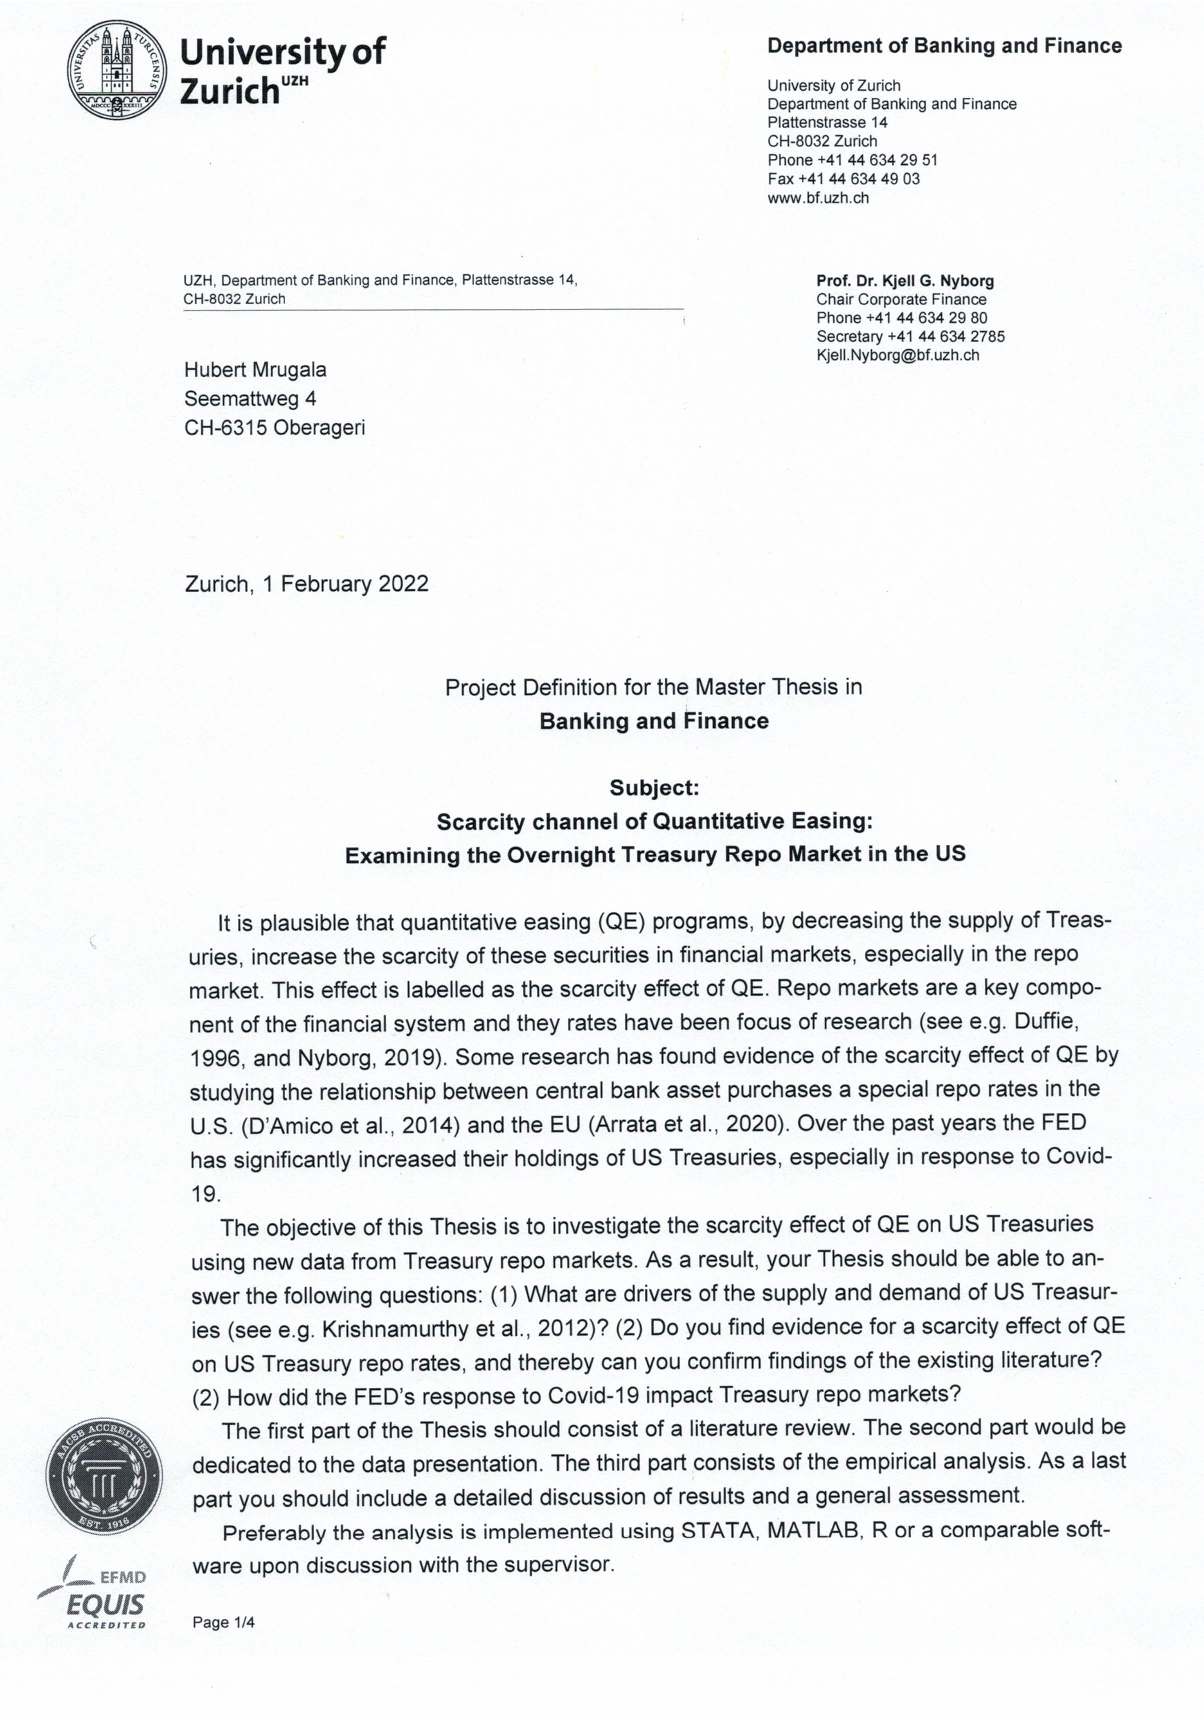
\includegraphics[page=1,width=.86\textwidth]{../../project_definition.pdf}
  \end{center}
\end{figure}
\newpage
\begin{figure}[h!]
  \begin{center}
    \includegraphics[page=2,width=.86\textwidth]{../../project_definition.pdf}
  \end{center}
\end{figure}
\newpage
\begin{figure}[h!]
  \begin{center}
    \includegraphics[page=3,width=.86\textwidth]{../../project_definition.pdf}
  \end{center}
\end{figure}
\newpage
\begin{figure}[h!]
  \begin{center}
    \includegraphics[page=4,width=.86\textwidth]{../../project_definition.pdf}
  \end{center}
\end{figure}

\thispagestyle{firststyle}
\newpage
\section*{Executive Summary}
\thispagestyle{firststyle}

\lipsum[1-3] % Here goes the text


\tableofcontents
\listoffigures
\listoftables
\newpage
\pagenumbering{arabic}

\section{Introduction}

\lipsum

\section{Mechanics of collateral}

\lipsum

\section{Drivers of a collateral spread}

\lipsum

\section{Empirical}

\subsection{Descriptive Statistics}

\lipsum

\subsection{Methodology}

\lipsum

\subsection{Base Model}

\lipsum

\subsection{Extension}

\lipsum

\section{Conclusions}

\lipsum

\newpage

\appendix
\noappendicestocpagenum
\addappheadtotoc
%\appendixpage

\renewcommand{\theequation}{A.\arabic{equation}}

[ You may also want to add an appendix, if it makes sense. You delegate proofs to the appendix or other material that is essential for the understanding of your work, but would distract the reader if placed in the main text... ]

\section{Proof of Proposition [...] }
[....], we can apply Ito's formula for Lévy processes   to obtain the
dynamics of the forward LIBOR $L(t,T_j)$ to obtain the
dynamics of the forward LIBOR $L(t,T_j)$ under the $T_{j+1}$-forward measure
as follows:
\begin{eqnarray}
\frac{dL(t,T_j)}{L(t,T_j)} &=& b (t,T_{j},T_{j+1}) dt +
\frac{1}{2} \lambda ^2(t,T_j) dt +
\frac{1}{2} V _t^W dt\nonumber \\
&+& \int_{-\infty}^{0}  \left[ e^{x}-1-x \right]
\pi_{J^-}^{\mathbb Q_{j+1}}(dx)\nu _t^J dt + \int_{0}^{\infty} \left[
e^{x}-1-x \right] \pi_{J^+}^{\mathbb Q_{j+1}}(dx)\nu _t^Jdt \nonumber \\
&+& \lambda (t,T_j) dB_{t}^{Q_{j+1}}+ \sqrt{ V _t^W}
dW_{t}^{Q_{j+1}}+ \int_{-\infty}^{0} \left[ e^{ x}-1 \right]
\left[ \mu^- (dt,dx) -
\pi_{J^-}^{Q_{j+1}}(x) dx \nu _t^J dt \right]\nonumber \\
&+& \int_{0}^{\infty} \left[ e^{ x}-1 \right] \left[ \mu ^+ (dt,dx)
- \pi_{J^+}^{Q_{j+1}}(x) dx \nu _t^J dt \right].
\end{eqnarray}
To ensure that $L(t,T_j)$ is a martingale under the
$T_{j+1}$-forward measure, the drift must equal zero, which gives the
drift condition in the proposition. $\blacksquare$

% \bibliography{refs}

\newpage
\thispagestyle{firststyle}
\section*{Eidesstattliche Erklärung}
Der Verfasser erklärt an Eides statt, dass er die vorliegende Arbeit selbständig, ohne fremde Hilfe und ohne Benutzung anderer als die angegebenen Hilfsmittel angefertigt hat. Die aus fremden Quellen (einschliesslich elektronischer Quellen) direkt oder indirekt übernommenen Gedanken sind ausnahmslos als solche kenntlich gemacht. Die Arbeit ist in gleicher oder ähnlicher Form oder auszugsweise im Rahmen einer anderen Prüfung noch nicht vorgelegt worden.\\[2cm]

\hspace{60pt} 18.05.2022

\dotbox{Ort, Datum} \hfill \dotbox{Unterschrift des/der Verfassers/in}
\end{document}
